%%%%%%%%%%%%%%%%%%%%%%%%%%%%%%%%%%%%%%%%%%
%% TEX main file for the CLAS12 Nim Papers
%%       Do not edit this file
%%%%%%%%%%%%%%%%%%%%%%%%%%%%%%%%%%%%%%%%%%
\documentclass[3p,times,twocolumn]{elsarticle}

\usepackage{lineno, hyperref, multicol, color, xspace, pdfwidgets, enumerate, amssymb, subfig, amsmath, gensymb, adjustbox}


\def \rarr {\rightarrow}
\def \grinp {\includegraphics}
\def \tw {\textwidth}

\modulolinenumbers[5]
\linenumbers

\journal{Nuclear Instruments and Methods A}

\begin{document}

\begin{frontmatter}
\title{CLAS12 High Threshold Cherenkov Counter}

\author[1]{Y.G.Sharabian}
\author[1]{V.D.Burkert}
\author[1]{S.Christo}
\author[1]{C.Cuevas}
\author[1]{H.Dong}
\author[13]{S.Danagoulian}
\author[2]{A.Ellis}
\author[1]{L.Elouadrhiri}
\author[1]{B.Eng}
\author[3]{K.Hafidi}
\author[4]{I.Illari}
\author[1]{G.Jacobs}
\author[5]{K.Joo}
\author[1]{D.Kashy}
\author[6]{A.V.Kubarovsky}
\author[1]{V.P.Kubarovsky}
\author[7]{S.Maiylian}
\author[1]{N.Markov}
\author[1]{M.Mcmullen}
\author[1]{B.Miller}
\author[8]{r.Niyazov}
\author[7]{R.Paremuzyan}
\author[9]{W.Phelps}
\author[1]{V.Popov}
\author[10]{A.Puckett}
\author[1]{B.Raydo}
\author[11]{D.Riser}
\author[12]{P.Stoler}
\author[13]{A.Vlasov}
\author[7]{A.Voskanyan}

\address[1]{Placeholder location}
\address[2]{Placeholder location}
\address[3]{Placeholder location}
\address[4]{Placeholder location}
\address[5]{Placeholder location}
\begin{abstract}

For the 12 GeV upgrade of Jefferson Laboratory, a Silicon Vertex Tracker (SVT) has been designed for the CLAS12 spectrometer using single-sided microstrip sensors fabricated by Hamamatsu. The sensors have a graded angle design to minimize dead areas and a readout pitch of 156 $\mu$m, with intermediate strips. Each double-sided SVT module hosts three daisy-chained sensors on each side with a full strip length of 33~cm. There are 512 channels per module, read out by four Fermilab Silicon Strip Readout (FSSR2) chips, featuring data-driven architecture, mounted on a rigid-flex hybrid board. The modules are assembled on the barrel using a unique cantilevered geometry to minimize the amount of material in the tracking volume. This paper is focused on the design, qualification of the performance, and experience in operating and commissioning the tracker during the first year of the data taking.

\end{abstract}

\end{frontmatter}

\date{\today}

\section{Overview}

simulations overview description, how geometry and digitization.

Then we go to each detector

- geometry
- calibration constants
- digitization.





\section{Requirements}

hallb requirements description


\section{Design}

The CLAS12 Trigger System was designed as a 3-stage pipeline-style system with total latency up to 8~$mu$s. Input information for the Trigger System comes from two sources:  Flash Analog to Digital Converters (FADCs) used in the photomultiplier tube (PMT)-based detectors, and Drift Chamber Readout Boards (DCRBs) used in Drift Chambers. The FADCs and DCRBs work as the pre-trigger level, reporting information to the Trigger System in the appropriate form. Stage 1 receives information from the FADCs and DCRBs and performs data processing according to the type of detector. Stage 2 performs a timing and geometry coincidence between different subsets of detectors in six groups, corresponding to the six-sector CLAS12 detector structure, as well as requires coincidence with information from central detectors. Stage 3 forms the final trigger decision. The CLAS12 Trigger diagram is shown in Fig.~\ref{fig:TriggerDiagram}.

\begin{figure}[hbt]
	\centering
	\includegraphics[width=1.0\columnwidth,keepaspectratio]{img/CLAS12_TRIGGER_1.pdf}
	\caption{The CLAS12 Trigger System diagram.}
	\label{fig:TriggerDiagram}
\end{figure}


\subsection{FADCs as Pre-trigger}

All PMT-based detectors in CLAS12 participating in the Trigger System use JLab VXS 250~MHz flash ADCs as the starting point of the trigger logic (FADC, \cite{daq-ref}). Each channel of the FADC boards is pre-programmed with gain, pedestal, and amplitude threshold above pedestal. Every pulse above amplitude threshold is integrated and sent to the corresponding section of the Stage 1 trigger logic. The 16-channel FADC boards report 13-bit pulse integrals and 3-bit pulse time every 32~ns, which allows the following trigger logic to restore 4~ns pulse resolution while the double pulse resolution remains 32~ns. Based on the FADC reporting schedule, the following trigger logic stages can work on a 250~MHz clock, although in that case we found it problematic to meet the Field Programmable Gate Array (FPGA) timing. Because of that, our Stage 1 algorithms run on 125~MHz or slower clocks as described below. Tteh trigger information is provided to the following stages using VXS backplane serial lines.


\subsection{DCRBs as Pre-trigger}

The Drift Chamber-based trigger uses JLab 125~MHz discriminator/TDC boards (DCRB, \cite{daq-ref}) to feed the Trigger System. These 96-channel units report hits above the pre-programmed thresholds every 16 ns. As for the FADC boards, the DCRBs are implemented in VXS format and provide trigger information using VXS backplane serial lines.


\subsection{Stage 1 Trigger} 

The Stage 1 trigger uses specially designed VXS Trigger Processor boards (VTP, see Section \ref*{sec:vtp_board}). The VTP boards are installed in switch slots in every VXS crate participating in the Trigger System. The VTPs collect trigger data from the pre-trigger boards (FADCs and DCRBs) over VXS serial lines.

The most complex processing is performed for the electromagnetic calorimeters (cluster finding) and the Drift Chambers (segment and road finding). In the following sections we describe the design of the various trigger components.


\subsubsection{Electromagnetic Calorimeters}
\label{sec:ECAL}

The CLAS12 electromagnetic calorimeter (ECAL, \cite{ec-ref}) includes two separate subsystems, the EC and PCAL. Each consists of multiple layers of scintillating strips and lead sheets with photomultiplier readout on one side of the scintillators (the PCAL is shown in Fig.~\ref{fig:PCAL}, the EC is similar). The primary purpose of these detectors is electron identification by defining the energy and coordinate of their electromagnetic showers, referred to as clusters. The cluster finding algorithm was well established during off-line data processing development, and was adopted for the trigger implementation with some simplifications.

The algorithm first searches for one-dimensional clusters in each of the three calorimeter views (u,v,w), sorting them by energy and keeping only those above threshold, with a maximum number of four clusters in each view. Next the algorithm searches for two-dimensional clusters looking for overlap between the three views. For all two-dimension clusters found, it performs attenuation corrections based on pre-loaded tables of the attenuantion lengths of the scintillation strips using the distance from the cluster to the PMT, to deternime the correct cluster energy. Finally, the algorithm sorts the two-dimension clusters by energy and reports those above threshold, with a maximum number limited to four. For every cluster, the energy and coordinates are reported to the Stage 2 trigger every 8~ns. There is a persistency parameter that allows the same clusters to be reported for several consecutive 8~ns intervals to check for a timing coincidence with the other trigger components, as well as a timing delay parameter for the same purpose. One event with a single cluster is shown in the PCAL (preshower calorimeter) in Fig.~\ref{fig:PCAL}. The corrected energies are shown for the individual strips.

It should be mentioned that such an algorithm is designed to find clusters with a maximum energy to target electron identification. For some CLAS12 experiments, it is necessary to identify minimum-ionizing particles (MIPs) using the same trigger component. For that purpose, clusters with energy below a certain defined threshold can be selected. Such a method works for events where the number of clusters does not exceed four, otherwise there is a risk of losing low-energy clusters corresponding to MIPs. Intensive trigger efficiency studies were conducted for such cases, and the MIP trigger efficiency was measured and found acceptable.

\begin{figure}[htp]
	\begin{center}
		\centering
		\includegraphics[width=7cm]{img/pcal1.png}
		%\includegraphics{PCA.pdf}
		\caption{Trigger System representation of a cluster reconstruction using the three views of the PCAL in one sector of CLAS12.}
		\label{fig:PCAL}
	\end{center}
\end{figure} 


\subsubsection{High Threshold Cherenkov Counter}
\label{sec:HTCC}

The CLAS12 High Threshold Cherenkov Counter (HTCC, \cite{htcc-ref}) serves as one of the primary components of the electron trigger logic. It was specially designed to discriminate electrons from other charged particles. The HTCC consists of 48 mirror sections readout by PMTs connected to FADCs (see Fig.~\ref{fig:multihitHTCC}). For trigger purposes, a 2x2 section sliding window is used to identify clusters. The cluster may include from one to four PMT signals collecting the Cherenkov light from the adjacent mirrors as shown in  Fig.~\ref{fig:multihitHTCC}. The configuration parameters include the single channel energy threshold, cluster multiplicity threshold, and cluster energy threshold. The results are reported to the Stage 2 trigger as 48-bit masks every 4 ns. The FADC ``gain'' configuration parameter allows for PMT energy calibrations, making it possible to set energy thresholds in terms of the number of photoelectrons.


\begin{figure}[htp]
	\begin{center}
		\centering
		\includegraphics[width=8cm]{img/multiHits.pdf}
		\caption{Hits registered by the HTCC (red circles) and the reconstructed cluster position (yellow). The hit position and cluster position coincide for one hit clusters (top left plot), which has the lowest position resolution.}
		\label{fig:multihitHTCC}
	\end{center}
\end{figure} 


\subsubsection{Drift Chamber}
\label{sec:DC}

The CLAS12 Drift Chambers (DC, \cite{dc-ref}) contain six superlayers in each of the six CLAS12 sectors. Each superlayer contains six layers, and 112 wires in each layer. There is no signal amplitude information available, only hit information can be used in the trigger. The Trigger algorithm was designed as a two-step process.

In the first step it searches for segments in each of the six superlayers, reporting a 112-bit mask with the bits set for the segments found. The search for segments is conducted based on a pre-loaded segment dictionary, generated by the Drift Chamber simulation software based on the wire locations in the superlayers. If several segments are found in the same location, the one with the maximum number of hits is kept. In theory, the number of layers contributing to each segment must be equal to 6, and the number of hit wires in a segment can vary from 6 to 12 depending on the track position and angle. In practice, the number of layers and hits in each segment can be less because of Drift Chamber inefficiencies and hardware problems, so the threshold for the segment finder in the trigger logic was usually set to 4 and sometimes to 3 layers out of 6 to ensure an efficient trigger.

After the segment search is complete and the six 112-bit masks are ready, the second step is performed, in which a pre-loaded road dictionary (corresponding to all possible charged particle trajectories) is used to identify possible track candidates (so-called road finding). The road disctionaries were generated by the GEMC Monte Carlo simulation program (\ref) or taken from the real beam data (\ref). At least five out of six superlayers are required to satisfy the trigger condition. All found roads are reported to the Stage 2 trigger every 16~ns. The information reported in the form of 112-bit words is used for the geometry match in the Stage 2 trigger.


\subsubsection{Forward Time-Of-Flight System}

The CLAS12 Forward Time-Of-Flight System (FTOF, \cite{ftof-ref}) contains two layers of scintillating counters in each sector, but only one layer is used by the trigger logic. This layer contains 62 counters with PMT readout on both ends. When both PMTs report a signal above threshold, the trigger system considers it as a hit. A 62-bit hit mask is reported to the Stage 2 trigger every 4~ns. The trigger logic configuration includes a single channel energy threshold and a counter average energy threshold (geometry mean). The FTOF participates in non-electron triggers such as the muon trigger.


\subsubsection{Central Time-Of-Flight System}

The CLAS12 Central Time-Of-Flight System (CTOF, \cite{ctof-ref}) consists of 48 scintillation counters, surrounding the target as a barrel, with PMT readout from both ends. Its trigger logic is similar to that for FTOF, with a 48-bit mask reported to the Stage 2 trigger every 4~ns.


\subsubsection{Central Neutron Detector}

The CLAS12 Central Neutron Detector (CND, \cite{cnd-ref}) consists of three layers of scintillation counters, installed radially outward from CTOF, with 24 counters per layer and 72 counters total. Its trigger logic is similar to that for FTOF and CTOF, with a 24-bit mask reported to the Stage 2 trigger every 4~ns (usually the inner layer only).


\subsubsection{Forward Tagger Calorimeter and Hodoscope}

The CLAS12 Forward Tagger Calorimeter and Hodoscope (FT, \cite{ft-ref}) trigger is designed to trigger on electrons at small forward angles (theta from 2deg to 5deg). The calorimeter is a stack of 332 lead tungstate crystals connected to avalanche photodiodes (APDs) that are readout by FADCs. The hodoscope consists of two scintillating fiber layers, each having 116 pixels (of two sizes) that matches the geometry of the calorimeter. The calorimeter trigger finds clusters by looking for a seed hit at each crystal location. If the deposited energy in a crystal is greater than the seed threshold and is a local maximum in space (using a 3x3 crystal view) and time, then it is considered a seed hit. For each seed hit, a cluster is formed by summing all of the energies centered on the seed hit in a 3x3 crystal view for all hit times coincident with the seed hit (up to $\pm$16~ns). The seed hit time, which due to time walk effects is the earliest hit in the cluster, is used for the cluster time stamp, providing a 4~ns resolution. The geometrically matched hodoscope pixels for both layers are checked for time coincident hits with the calorimeter seed hit and the cluster is tagged as having none, layer 1, layer 2, or both layers of the hodoscope present. Found clusters are serialized and streamed to the Stage 2 trigger where several programmable trigger cuts can discriminate clusters based on energy, charge, and multiplicity.


\subsection{Stage 2 Trigger}

The Stage 2 trigger collects data from Stage 1 using fiber optics. It is based on the number of SubSystem Processor boards (SSP, see Section \ref*{sec:ssp_board}) all installed in one VXS crate. After receiving the Stage 1 trigger streams, the SSPs form subsystem coincidences for the six identical sets of forward detectors (called sectors) and the central detectors (all separately). Each subsystem trigger stream goes through a programmable delay that provides 4~ns resolution when deskewing to optimize the time coincidence. Next follows a programmable coincidence window for each subsystem trigger stream, also with a 4~ns step resolution, to ensure that the different subdetector signals will remain stable long enough to form a time coincidence regardless of jitter due to particle time-of-flight, detector response, and trigger jitter. Stage 2 Trigger specifications are shown in Table~\ref{tab:stage_2_specs}.

\begin{table}
\begin{center}
	\begin{tabular}{| l | l |}
		\hline \hline
		Name				& Specification	\\
		\hline
		Latency (Stage 1+2)		& 5~$\mu$s	\\
		Jitter				& 4~ns		\\
		Stage 2 trigger bits		& 8		\\
		Deskew range			& 4~$\mu$s	\\
		Deskew step size		& 4~ns	\\
		Coincidence window range	& 2~$\mu$s	\\
		Deskew step size		& 4~ns	\\
		\hline \hline
	\end{tabular}
\end{center}
\caption{Stage 2 Trigger Specifications}
\label{tab:stage_2_specs}
\end{table}

The forward detectors in the trigger consist of FTOF, EC, PCAL, HTCC, and DC. A single SSP collects all forward detector trigger streams from a single sector of CLAS12. After the delay and concidence widths are applied to each input stream, the input streams are copied to 8 programmable sector trigger bits. Each sector trigger bit contains a variety of trigger primitives and customizeable thresolds/cuts that can be tailored for a particular trigger type. The sector trigger bits are computed and sent to the final Stage 3 trigger. Forward Detector Trigger primitives are shown in Table~\ref{tab:fd_trig_primitives}.

\begin{table}
\begin{center}
	\begin{tabular}{| l | l |}
		\hline \hline
		Primitive Name			& Trigger Bit Parameters	\\
		\hline
		PCU     			& Mask				\\
		FTOF    			& Mask				\\
		PCAL				& Cluster Emin, Emax		\\
		ECAL				& Cluster Emin, Emax		\\
		PCAL+ECAL			& Cluster Emin			\\
		HTCC				& Mask				\\
		{\bf Geometry Matched}		&				\\
		PCUxFTOF			& Bar match tolerance		\\
		PCALxDC				& Cluster Emin			\\
		\hline \hline
	\end{tabular}
\end{center}
\caption{Forward Detector Trigger Primitives}
\label{tab:fd_trig_primitives}
\end{table}

The central detectors participating in the trigger consist of CTOF, CND, and FT. A single SSP collects all central detector trigger streams. After the delay and concidence widths are applied to each input stream, the input streams are copied to 8 programmable central trigger bits. Each central trigger bit contains a variety of trigger primitives and customizable thresolds/cuts that can be tailored for a particular trigger type. The central trigger bits are computed and sent to the final Stage 3 trigger where all sector and central trigger bits arrive to compute the global trigger bits. Central Detector Trigger primitives are shown in Table~\ref{tab:cd_trig_primitives}.

\begin{table}
\begin{center}
	\begin{tabular}{| l | l |}
		\hline \hline
		Primitive Name			& Trigger Bit Parameters	\\
		\hline
		CND     			& Mask				\\
		CTOF    			& Mask				\\
		FT				& Cluster Emin, Emax, 		\\
						& Cluster Size, Hodoscope	\\
		{\bf Geometry Matched}		&				\\
		CNDxCTOF			& Bar match tolerance		\\
		\hline \hline
	\end{tabular}
\end{center}
\caption{Central Detector Trigger Primitives}
\label{tab:cd_trig_primitives}
\end{table}


\subsection{Stage 3 Trigger}

The Stage 3 trigger is the final stage and collects all sector and central trigger bit streams in a single module where they can be combined in a variety of ways to generate the global trigger bits used for reading out the Data Acquisition System (DAQ). It is implemented on a single VTP board installed in the switch slot on the same VXS crate where all Stage 2 trigger SSPs reside. There are 32 independent trigger bits that can form a trigger based on any combination of sector and/or central trigger bits. Each trigger bit contains two sector trigger bit conditions (required to both be true) and a signle central trigger bit condition. Additionally, each trigger bit contains a 16~bit prescaler, final pulse width, and scaler. Stage 3 Trigger specifications are shown in Table~\ref{tab:stage_3_specs}.

\begin{table}
\begin{center}
	\begin{tabular}{| l | l |}
		\hline \hline
		Name				& Specification	\\
		\hline
		Latency (Stage 1+2+3)		& 7~$\mu$s	\\
		Jitter				& 4~ns		\\
		Stage 3 trigger bits		& 32		\\
		Prescaler			& 0-65535	\\
		Trigger bit width		& 4~ns - 1~$\mu$s	\\
		Pulse rate			& 0.05~Hz - 125~MHz	\\
		\hline \hline
	\end{tabular}
\end{center}
\caption{Stage 3 Trigger Specifications}
\label{tab:stage_3_specs}
\end{table}


\subsection{Trigger Information in Data Stream}
\label{sec:trigger_in_datastream}

An important part of the Trigger System is the Event Builder, which allows the trigger components to participate in event-by-event readout the same way as is done for the DAQ components. All three stages of the Trigger System are equipped with Event Builders. Every time the CLAS12 DAQ is triggered, Stage 1 will build the data bank(s) with trigger decision details (such as the ECAL cluster coordinate/energy or DC segments/roads information), Stage 2 will build the data bank with sector-level and central detector coincidence results, and Stage 3 will build the data bank that contains the trigger bit decisions for all final 32 trigger bit decisions. Event Builders read information from the pipeline-style buffers for a given programmable window related to the readout trigger time. All trigger-related data banks are available in the data stream along with the DAQ data banks, providing detailed information about the trigger decision for every accepted event. In particular, this allows the Trigger System to be run in ``tagging mode'', which is a powerful way to test the trigger efficiency (using either a loose or a random trigger).

\section{Hardware Components and Constructions}

template Hardware Components and Constructions description


\section{High Level Synthesis in CLAS12 Trigger System development} sergey

\subsection{Our motivation to use HLS}

HLS makes it easier to incorporate well-established data processing algorithms, typically written in C++ or other high-level language, into FPGA-based projects.
It allows to involve programmers who developed algorithms for offline data processing but with limited FPGA programming experience. It also makes it possible to validate code inside offline processing framework.

\subsection{Trigger components implemented with HLS}

HLS was used to develop most of stage 1 components of CLAS12 trigger:

\begin{itemize}
	\item High Threshold Cherenkov Counter (cluster energy reconstruction)
	\item Forward and Central Time-of-Flight Counters (clustering and left-right correction)
	\item Electromagnetic and Preshower Calorimeters (cluster energy and position reconstruction)
\end{itemize}

Time-of-Flight and Cherenkov counters implementation was rather trivial, it would typically takes less then 10-15\% of the Virtex 7 chip and timing requirements were easily met.

Calorimeter trigger implementations required much more effort because of its complex nature which requires significant FPGA resources. Details are further explained in the next sections using Electromagnetic Calorimeters as the example.


\subsection{CLAS12 Electromagnetic Calorimeters}

Among all trigger system elements, the most challenging for FPGA implementation was trigger component serving two CLAS12 electromagnetic calorimeters. Due to its structure, those calorimeters do not provide cluster coordinates or energies without significant event reconstruction. Both calorimeters consists of three sets of scintillation strip layers with PMT readout on one side of strip. To reconstruct clusters it is needed to find peaks in all three layers, find crosses of those peaks, apply attenuation length corrections to individual scintillation strips, correct peaks energies, correct clusters energies, and finally report clusters coordinates and energies to the following stage of the trigger system. Cluster reconstruction procedure was developed before as part of offline analysis and was well established, so we decided to use it as starting point for trigger component design.

Event with single cluster is shown in
CLAS12 PCAL (preshower calorimeter); corrected energies are shown for individual strips

\subsection{HLS Settings}

Clock uncertainty is set as 30\% of main clock, we found that it forces HLS to produce more realistic timing estimates. A single HLS project often cannot exceed several percent of FF and LUT budget, otherwise it may be a problem to meet timing requirement on VIVDO implementation step. Typical project from Calorimeter trigger is shown below.

\subsection{VIVADO Settings}

Common settings were used as shown on picture below. It usually takes 3+ hours to compile Calorimeter project on Dell R730 server under RHEL7. For some firmware versions, we were able to utilize 100\% of LUTs and still meet timing – if clock domain was 125MHz or lower.

\subsection{Firmware validation for HLS-based projects}

The ability to validate firmware using C++ implementation is the one of the biggest advantages of HLS. During the course of development and commissioning we ran HLS C++ code on simulated and real data from CLAS12 detectors, implementing required features and fixing bugs. During data taking we were able to find and fix observed problems or add new features in several hours, which was very important to save beam time.

\subsection{Our conclusion about HLS Usage}

CLAS12 Calorimeters and other detectors were successfully implemented into trigger system using HLS to produce core part of the firmware. This trigger was used in the first physics run and worked as expected. We were able to select events based on individual cluster energy, something which was possible before only during offline data processing.
HLS in general appears to be a useful tool, especially to implement smaller trigger components like Cherenkov or time-of-flight counters. For components utilizing significant portion of the FPGA, it will be great to improve HLS in following directions:

\begin{itemize}
	\item Support multi-clock domains
	\item Improve subroutine calls by allowing option to fully registered paths between modules. 
	\item Improve state machine logic, for example support streams between routines inside the project and be able to generate separate state machines for separate routines. It will allows to avoid splitting project manually and use HDL as top interface as we are currently forced to do.
\end{itemize}

\section{Software}



\subsection{Development Software}

Several software packages were used to implement and test the trigger logic developed for CLAS12. These were the FPGA synthesis and implementation, FPGA high level synthesizer, and FPGA simulation software packages.

For FPGA synthesis and implemenation Xilinx ISE/Planahead and Vivado were used. Most of the front-end boards were developed years ago and use Virtex 5 and Spartan 6 FPGAs, which are not supported by Xilinx Vivado, so we relied on Xilinx ISE/Planahead for synthesis and implementation. Even though these tools are no longer updated by Xilinx they have proved to be stable, reliable, and deliver consistent results. Newer design use Xilinx 7-series parts (we used Artix, Kintex, and Virtex) so we used the Vivado tools, which had far better support than ISE/Planahead.

Vivado HLS was used to implement a variety of trigger algorithms, event builder logic, and general purpose logic. HLS components were able to be verified with C/C++ test benches on their own without anything more than GNU GCC and associated C/C++ header files from the HLS toolchain. This tool often allowed for faster implementation for FPGA implemenation, but many components still were implemented in HDL were resource and/or timing requirements become critical.

A cycle accurate simulation was setup to model, test, and debug the full trigger system was setup using Aldec Riviera. Using this tool we were able to perform simulations using the full trigger system in a mixed language environment (VHDL, Verilog, C/C++) for all FPGA componenets (Xilinx series 5, 6,and 7 components). VHPI was used to interface external C/C++ programs from the DAQ to the VHDL testbench. Using VHPI, calls to the DAQ EVIO C/C++ libraries were possible from VHDL making it possible to feed detector waveform data into the trigger simulation directly from monte-carlo and beam data files. Simulation intensive components, such as SerDes components, were replaced with fast and simple models once verified to improve the performance. The simulator is single-threaded and requires a license for each running instance, making it cost prohibitive to parallelize. Even so, it was capable processing 1 event every ~30 seconds on a typical desktop PC simulating the forward and central trigger system comprised of 24,192 drift chamber wires and ~3400 FADC250 channels.


\subsection{Operating Systems} Moffit

Stage 1 and stage 3 of the CLAS12 Trigger System controlled through Arch Linux running in Xilinx arm ...

Stage 2 controlled by CentOS Linux running on Intel controller. As results all 3 stages designed to provide convenient access to ...
using c/c++ programs.


Archlinux with armv7

\begin{itemize}
\item Linux Kernel 4.4.0
  \begin{itemize}
  \item Updates with specific support for Xilinx products
  \item Availaable at https://github.com/Xilinx/linux-xlnx.git
  \item Custom device-tree
  \item Provides FPGA programming interface
  \item Allocates Physical Memory for use with DMA and event buffers.
  \item Standard I^2c and SPI API.
  \end{itemize}

\item Archlinux compiled for armv7
  \begin{itemize}
  \item Available at https://archlinuxarm.org/
  \item Filesystem over NFS.
  \item diskless booting using tftp
  \end{itemize}

\end{itemize}



\subsection{Configuration Software}

\subsubsection{Configuration Files} sergey

CLAS12 Trigger system has large amount of parameters controlling its logic. Those parameters are set by writing values to hadrware registers, and controlled by reading those registers back. System is using ascii files, example is shown on (Fig.). Every line contains key word and the number of corresponding parameter values. Directive 'include' allows to use hierarhical set of configuration files. Normally main configuration file is selected during run startup procedure, and run control software resolves all 'include' directives creating one big configuration file. That file is used to program all trigger harwdare registers, and it is also written to the data stream for bookkeeping purposes. Register contents are read back and results recorded into data stream as well, providing full control of trigger system settings. Normally the same configuration files contains DAQ settings as well, makeing it complete source for entire DAQ/Trigger system settings.


\subsubsection{Timing Setting}

\begin{figure}[hbt]
	\centering
	\includegraphics[width=1.0\columnwidth,keepaspectratio]{img/delay_scan_ctof_ft.png}
	\caption{CTOFxFT Delay Scan}
	\label{fig:delay_scan_ctof_ft}
\end{figure}

One of the important components of the trigger setting process is delay curves measurements. For that purpose software procedure was developed. It includes special trigger configuration file and software tools to sweep individual subsystem latencies, record set of beam current normalized scalers, and produce corresponding delay plots Fig.~\ref{fig:delay_scan_ctof_ft}. Time trigger time setting detector was kept at a constant value, which determined the DAQ readout window timing, while the other subsystems were changed step by step to monitor the delay curve. Delays and coincidence widths were adjusted to account for known jitter sources to ensure no events are lost due poor timing alignment. This procedure was repeated every time trigger logic was changed.


\subsubsection{Gain calibration and Threshold settings}

One of the important settings in trigger system is FADC ones. As it stated above FADC boards serves as initial stage of the most of the Stage 1 trigger components (except Drift Chamber), and correct pedestal and gain calibration is critical for correct trigger system performance. Pedestal and gain measurements were conducted before run startup, and values were loaded using configuration files. As result, all thresholds in configuration files were set using understandable units such as MeV for calorimeters and the number of photoelectrons for cherenkov counter.

\section{Simulation}

A realistic model of the LTCC has been developed, describing the location and material composition
of the support box, the mirrors, PMTs, Winston-Cones, magnetic shields and the $C_4F_{10}$ gas, see \cite{gemc2019}.
A 3D view of the simulated geometry of the LTCC is shown in \F{simOverview}.


\begin{figure}
	\centering
	\includegraphics[width=0.99\columnwidth,keepaspectratio]{img/simOverview.png}
	\caption{The Geant4 model of the LTCC implemented in GEMC \cite{gemc2019}. This setup corresponds to the
             initial LTCC configuration for the first CLAS12 production running in spring 2018
			 where the LTCC sectors 2, 3, 5 and 6 were present. In this picture the hyperbolic mirrors and some magnetic shields
             in sector 3 (upper right) have been made transparent to show details of the Winston cones (grey) and magnetic shields (black).}
	\label{fig:simOverview}
\end{figure}

\subsection{Geometry}

The Cherenkov light is emitted on a small cone around the direction of the emitting particle. The polar angle of
the particles entering the LTCC can be different from the polar angle at the production vertex due
to the bending of the tracks inside the toroidal magnetic field.
Instead of having two sets of mirrors, one aligned for in-bending (toward the beamline) and one aligned for
out-bending (away from the beamline) particles, the optics of the mirrors was designed to maximize the
light collection of optical photons originating from the target (placed at the center of the CLAS12 coordinate system),
to average the cases for the two charged particles.

The mirror shapes were described mathematically by ellipsoidal and hyperbolic curves.
The ellipsoid first focal point is the target location and the second focal point was chosen
to place the mirrors as far back in the box as possible to maximize the amount of gas seen by the tracks.
The second ellipsoid focal point overlaps with the hyperbolic first focal point. The hyperbole shape was optimized to focus the light
collection on PMTs placed on the shadow of the torus magnet coil, near the LTCC box walls, see \F{mirrorMath}.


\begin{figure}
	\centering
	\includegraphics[width=0.98\columnwidth,keepaspectratio]{img/mirrorMath1.png}
	\includegraphics[width=0.98\columnwidth,keepaspectratio]{img/mirrorMath2.png}
	\caption{The geometry of the LTCC mirrors is defined my the mathematical equations of the ellipse and hyperbola.
             Top: the ellipsoidal curve (solid line), with its center (square) and its focal points
             (circle at the origin, representing the target, and the bottom star).
             The two hyperbolas curves, defined by the two focal points (stars, one coinciding with the ellipse
			 focal point and the other at the desired location of the PMT) are the dashed lines. The
			 hyperbola at the bottom is the one that define the hyperbolic mirror.
             Bottom: zoomed in details of the setup above. The squares represent the mirrors left and right edges.
             These parameters are stored in databases and loaded in the software modeling the LTCC mirrors
             in the GEMC simulation \cite{gemc2019}.}
	\label{fig:mirrorMath}
\end{figure}

In the Geant4 implementation the elliptical mirrors are produced in three steps, each a boolean operation of volumes:

\begin{enumerate}
	\item make ellipsoidal mirror shells: by subtracting of two ellipsoidal volumes, rotated and centered on their designed position.
	\item cut out the mirrors from the shells: subtraction of the shells with left, right, top, and bottom boxes.
	\item place cut out mirrors: rotate and place the mirrors in the final position within the LTCC mother volume.
\end{enumerate}

The hyperbolic mirrors are made by Geant4 ``polycons'' that approximate the shape of the mirrors using a number of facets
varying from 10 (smallest mirror) to 30 (longest mirrors). The measured reflectivity is included in the simulation as
an optical property of the mirror material.

The CAD engineering models of the WCs have been used in the simulations, see \F{wcSimulation}.
The measured reflectivity is included in the simulation as an optical property of the WC material.
The WC and the PMT volumes are surrounded by boxes of mu-metal that model the LTCC magnetic shields, see \F{simShield}.

\begin{figure}
	\centering
	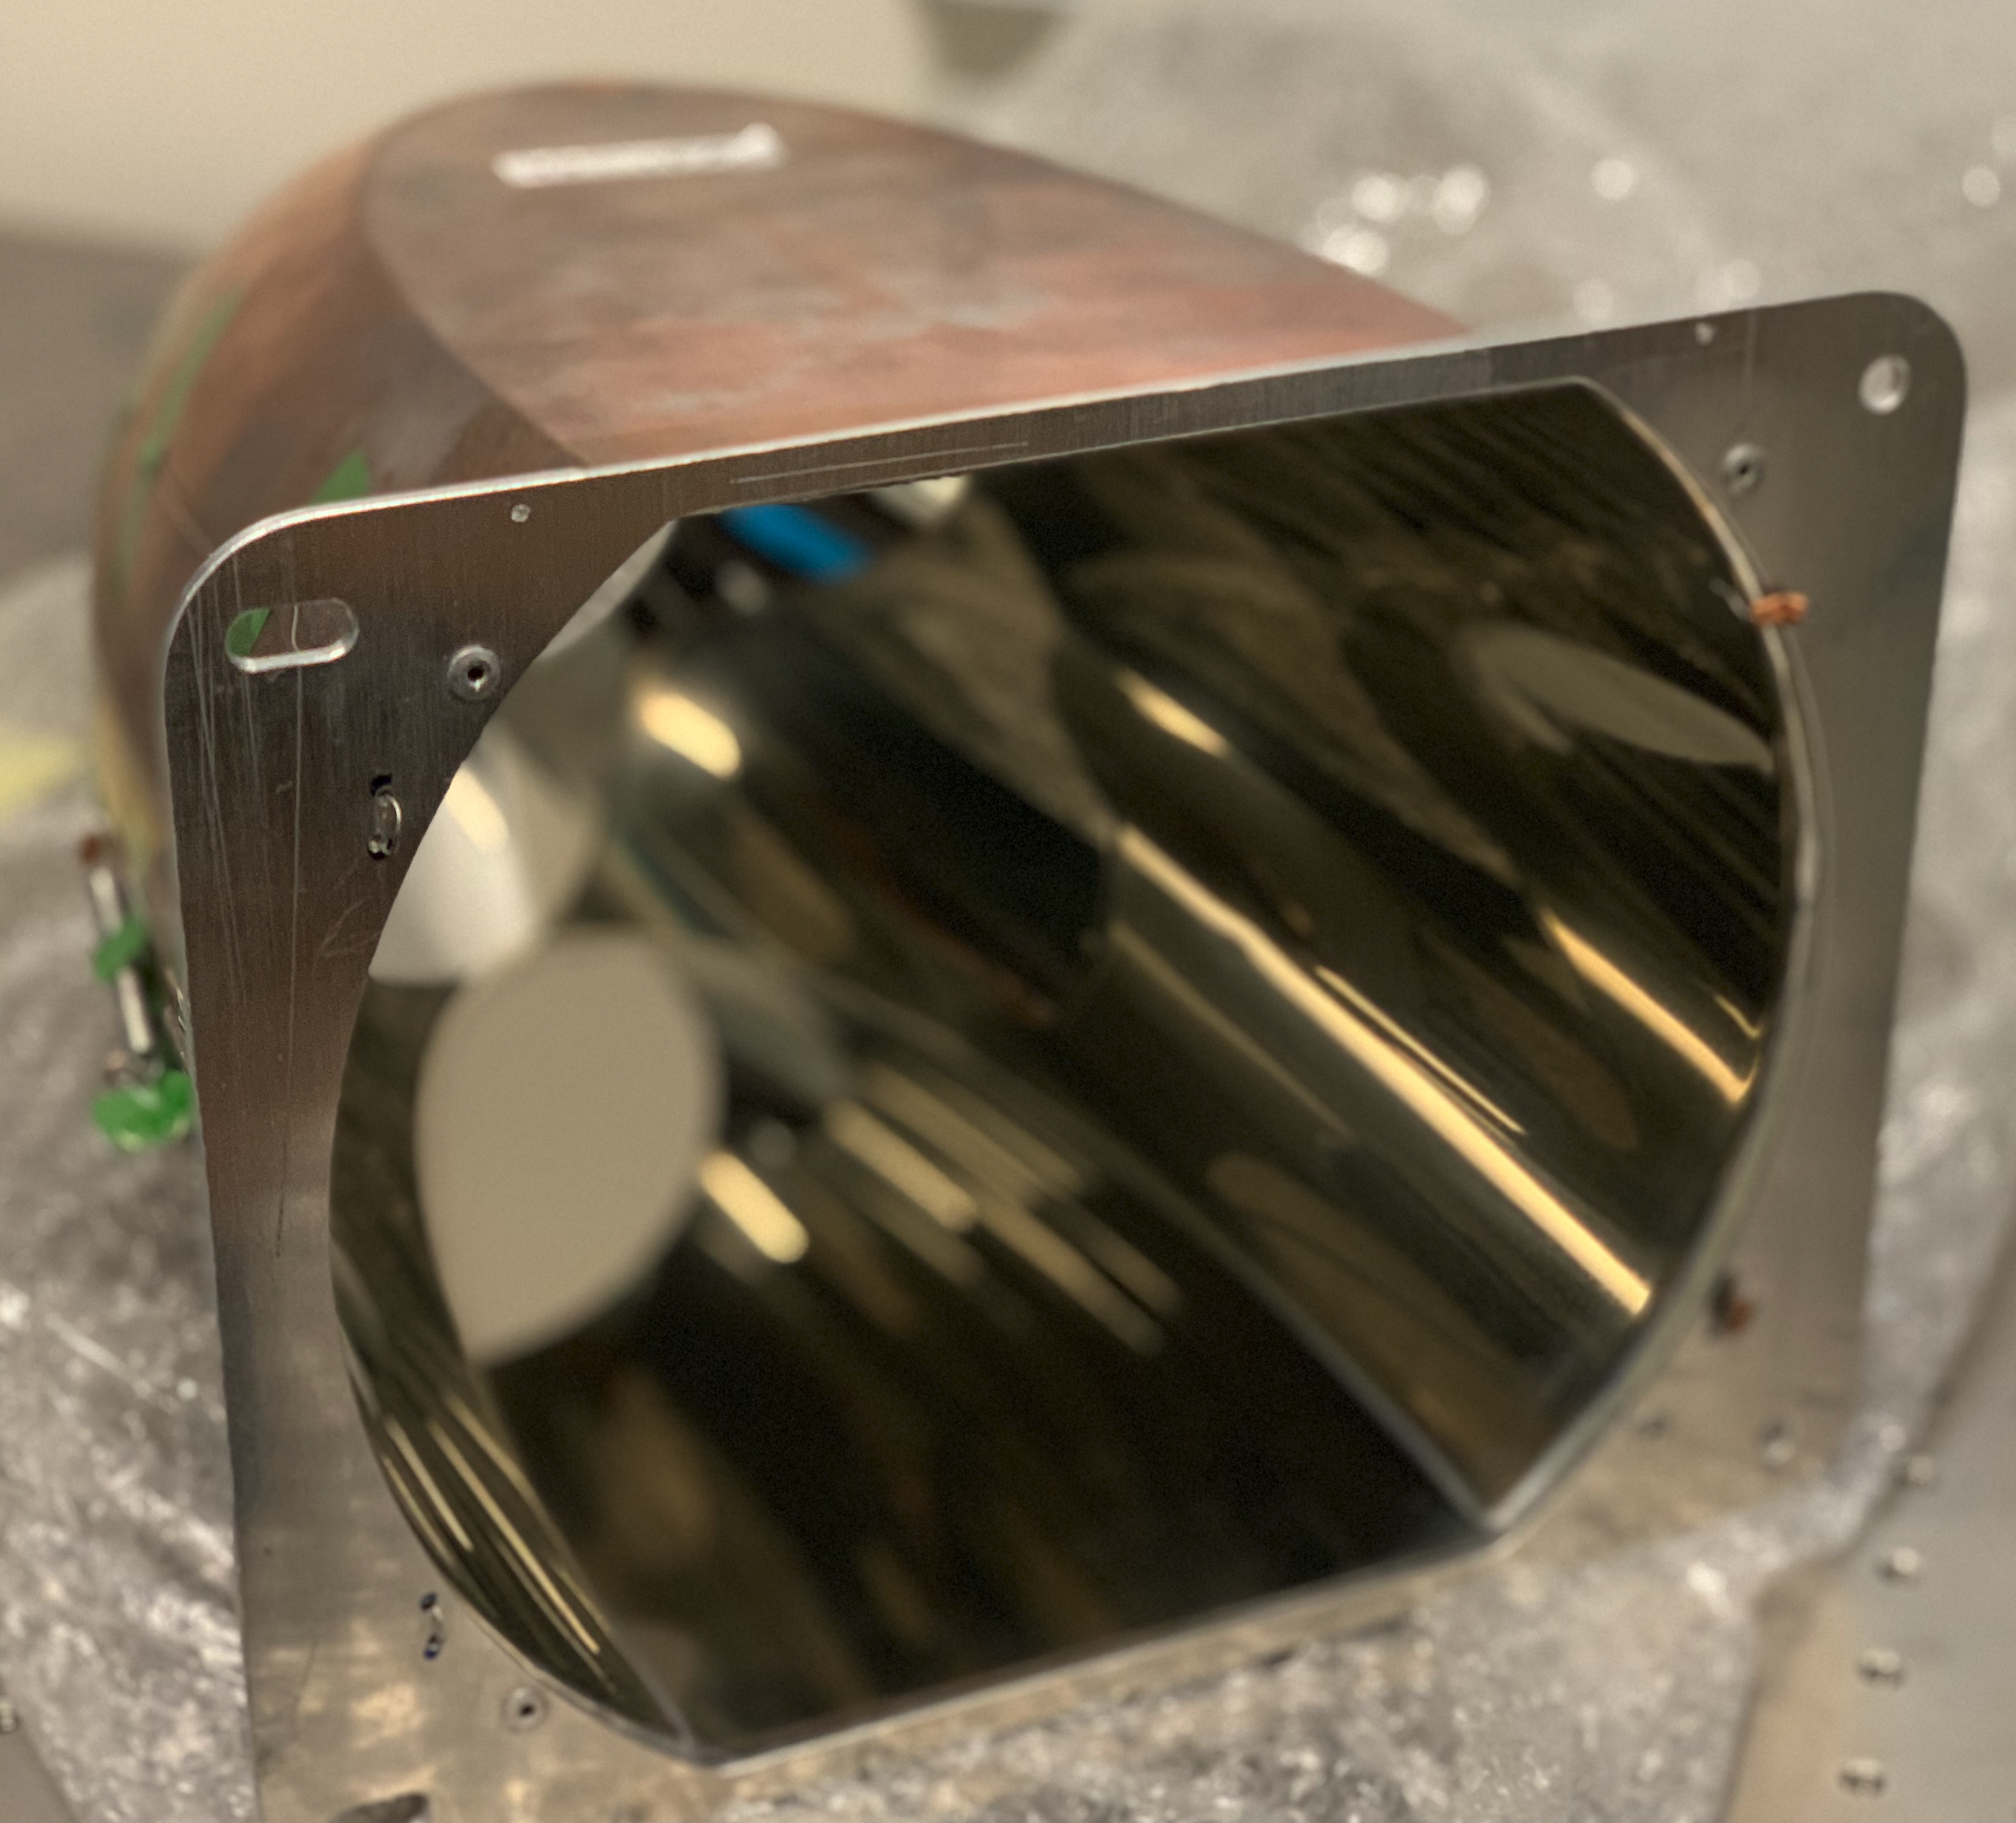
\includegraphics[width=0.99\columnwidth,keepaspectratio]{img/wcLargeReal.png}
	\includegraphics[width=0.99\columnwidth,keepaspectratio]{img/wcLargeSim.png}
	\caption{Top: a photograph of the large WC used for segments 12 to 18. Bottom: the tessellated volume used in the
            simulation, imported from the CAD engineering model.}
	\label{fig:wcSimulation}
\end{figure}

\begin{figure}
	\centering
	\includegraphics[width=0.99\columnwidth,keepaspectratio]{img/simShield.png}
	\caption{The magnetic shields are modeled by mu-metal boxes in the GEMC simulations (black). The WC (grey) focus the light on the red PMT surface.}
	\label{fig:simShield}
\end{figure}


The LTCC box support structure was imported from the engineering model shown in \F{boxCut}. This includes the 1-cm thick aluminum
elliptical and hyperbolic mirror support flanges, the nose, and the hardware mount to the CLAS12 beamline.


\subsection{Digitization}

In the digitization the number of collected photons is converted to charge by taking into account:

\begin{itemize}
	\item The quantum efficiency of the PMTs
	\item The position and width of the single photo-electron peak as stored in the CLAS12 calibration database
\end{itemize}


\subsection{Run Period Variations}

As the start of CLAS12 beam operations, there was not sufficient $C_4F_{10}$ gas to fill all sectors, so some LTCC sectors
where removed from the Forward Carriage. As they were installed or removed, any gas leaks were found and fixed.
These CLAS12 configuration changes are imported in GEMC as database variations of the simulation setup.
The default simulations only include sector 2 (S2), S3, S5, and S6 as the RICH detector replaces the LTCC S1 and S4.
The variations are listed in Table \ref{tab:simVariations}.

\begin{table}
	\begin{center}
		\begin{tabular}{| l | c |}
			\hline \hline
			Run Period       & Sectors Installed and Gas \\
			\hline
			Default          & S2, S3, S5, S6, all $C_4F_{10}$    \\
			RGA Spring 2018  & S2, S3, S6 (N$_2$), S5 ($C_4F_{10}$)  \\
			RGA Fall 2018    & S3 ($C_4F_{10}$), S5 (N$_2$)          \\
			RGB Spring 2018  & S3 ($C_4F_{10}$), S5 ($C_4F_{10}$) \\
			\hline \hline
		\end{tabular}
	\end{center}
	\caption{LTCC simulation variations for different CLAS12 run periods. Shown are which sectors are present and the gas in each sector}
	\label{tab:simVariations}
\end{table}







\section{Trigger system firmware development}

After trigger system design was complete and hardware components entered production stage firmware development was started. Both HLS and VHDL tools were used. Work was performed using data samples generated by GEMC/GEANT4, and using cosmic data when hardware components were installed. Present section describes those procedures. Validation on beam described in \ref{sec:validation}.

\subsection{Development using simulated data}

Development process consists of several methods and depends on the nature of the trigger component. Most stage1 components were implemented using HLS/VIVADO tool, where firmware was written using HLS C++ extension. In that case it was possible to develop and validate firmware as part of offline reconstruction framework using regilar desktop. Usually the offline processing alghorithms were re-written using HLS/C++, with appropriate simplification and structural changes to make it sutable for FPGA firmware. Input data for development were generated by GEMC/GEANT4. Generated data were processed directly by HPS/C++ code and compared with initial similation parameters. In addition, the same samples were processed by offline reconstruction software and results compared with the trigger output. That double check method practicaly guarantees bug-free implementation. It was no single case when C++ implementation passed tests on simulated data and failed on final validation stage. Most complicated stage1 components were developed and tested using this method.

Some stage1, as well as all stage2 and stage3 components were implemented using VHDL. For those, VIVADO tools were used for development and testing diring design phase, in particular ...
Generated data were feeded ...

\subsection{Development and validation using cosmic data}

When hardware components for CLAS12 detector were produced and mostly installed, and first version of firmware was ready for testing, all three trigger system stages firmwares were loaded and development continues for entire trigger system using cosmic data. At that point we started to perform trigger system validation for some components, while development was continue for others, as described in following sections.

\subsubsection{Alternative 'hit-based' trigger system}

CLAS12 detector inheritated some components from previously existed CLAS detector, in particular its trigger system. That system was feeded by tdc/discriminator boards and was able to produce 'hit-based' information only. We desided to keep it for reference purposes as alternative for the new trigger system. It was used during cosmic data CLAS12 detector calibration and new trigger system validation up to the point when new trigger system was ready. It is still operational and can be used to double-check of the main CLAS12 trigger system if needed.

\subsubsection{Development and validation of EC/PCAL special purpose trigger with cosmic data}

First step in cosmic data usage was detectors calibration. It was performed for all CLAS12 detectors and described in corresponding articles. Here we will describe, as an example, one of the procedures related to EC/PCAL calibration needed for correct trigger system performance. Similar procedures were executed for all detectors participating in trigger system.

Efficiency and spatial uniformity of cluster finding trigger in EC/PCAL described in Section 5.3 requires already calibrated calorimeters with pre-determined PMT gain and light attenuation constants loaded into the VTP/FPGA trigger firmware.  Calibration runs using a special purpose MIP trigger were used to obtain these constants. For that purpose so-called "pixel trigger" was developed and loaded into stage1 firmware along with main trigger, so it was possible to calibrate the system using pixel trigger and then switch to the main one for data taking. This "pixel trigger" used a simple multiplicity condition on 1D cluster size for each U,V,W view to reject undesirable muon trajectories and select normally incident tracks.  This reduced the trigger and data rate by 95$\%$ and ensured the same MIP energy was deposited for all possible triple intersections of single strips.

The pixel trigger pipeline executes these steps in parallel, with user configurable parameters in bold:
  1) If FADC hit energy $>$ \textbf{EMIN}, make a pulse \textbf{HITWIDTH}*4ns for that strip.
  2) Look for coincidence of U,V,W pixel strip candidates from step 1.
  3) Evaluate multiplicity \textbf{EVALDELAY}*4ns clock cycles after the leading edge of a candidate pixel from step 2.
  4) Generate pixel trigger if multiplicity requirement is met and we still have a hit on U,V,and W. 

Additional configurable trigger elements were introduced, including a total energy sum threshold \textbf{ESUM} and a lookup table for triplets of strips which satisfy the geometrical constraint $dU+dV+dW=\textbf{DALITZ}$, where $d$ is the normalized distance to the hit strip indicated by the arrows in Fig. 6 and $\textbf{DALITZ}=2$ for perfect pixels.  The latter test was sometimes necessary to prevent noisy PMTs from saturating the multiplicity (N=3) trigger condition.  Offline analysis showed that about $90\%$ of pixel triggers satisfied the Dalitz test (Fig. 7), while adjacent calorimeter elements which did not use the trigger had a much smaller pixel fraction.  This suggests the pixel trigger helps to suppress events which undergo multiple scattering, which would trigger adjacent strips and violate the multiplicity requirement.
%%%%%%%%%%%%%%%%%%%%%%%%%%%%%%%%%%%%%%%%% F I G U R E %%%%%%%%%%%%%%%%%%%%%%%%%%%%%%%%%%%%%%%%%%
\begin{figure}[!htb]
 \centering
  \includegraphics[width=0.95\columnwidth,keepaspectratio]{img/TwoClusters.png}
 \caption{Examples of clusters from cosmic muon triggers.  Desired trajectory (left) is normally incident on the face of PCAL and satisfies the single pixel multiplicity condition (N$_u$=N$_v$=N$_w$=1) in the FPGA pixel trigger.  Event at right shows a more vertical trajectory rejected by this trigger.}
\end{figure}
%%%%%%%%%%%%%%%%%%%%%%%%%%%%%%%%%%%%%%%%% F I G U R E %%%%%%%%%%%%%%%%%%%%%%%%%%%%%%%%%%%%%%%%%%

%%%%%%%%%%%%%%%%%%%%%%%%%%%%%%%%%%%%%%%%% F I G U R E %%%%%%%%%%%%%%%%%%%%%%%%%%%%%%%%%%%%%%%%%%
\begin{figure}[!htb]
 \centering
  \includegraphics[width=1.0\columnwidth,keepaspectratio]{img/PixelFraction.png}
 \caption{Offline analysis of events which satisfied the pixel trigger on ECINNER calorimeter.  Left plot shows 89$\%$ of ECINNER triggers satisfied the pixel test $dU+dV+dW=2$.  Right plot shows only 14$\%$ of the ECINNER triggers found an ECOUTER event that satisfied both the $N=3$ and pixel test. }
\end{figure}
%%%%%%%%%%%%%%%%%%%%%%%%%%%%%%%%%%%%%%%%% F I G U R E %%%%%%%%%%%%%%%%%%%%%%%%%%%%%%%%%%%%%%%%%%

\subsubsection{Development and validation of entire trigger system with cosmic data} 

While stage1 trigger components were validated separately from each other on development stage, stage2 and stage3 components requires entire system to be assembled to perform validation. Initially those two stages were programmed with simplified alghorithms to test signals propagation and basic trigger system functionality, only timing coincidense between different detectors was implemented. Development of stage2 and stage3 continues during cosmic run operations and later with beam operations, adding geometrical match between different detectors and increasing coincidense logic complexity.

\subsubsection{Trigger system flexibility and 'permanent development' mode}

Initial plan was to develop trigger system firmware which will satisfy all CLAS12 experiments for entire course of CLAS12 operation, meaning high (close to 100\%) trigger efficiency and reasonable purity. As the power and flexibility of the trigger system was revealed to community, additional requirements were placed to improve system purity, and to include additional physics processes. As result stage2 and stage3 components of the trigger system were under constant development during first year of CLAS12 operation, firmware was upgraded and entire system validated after every change. After a while trigger system reached the point when relatively small improvement in trigger purity can be achieved with significant efforts, after that development was declared complete. The nature of the fpga-based trigger system allows almost endless improvements, but such 'permanent development' mode seems not practical.


\section{Physics Triggers}
\label{sec:physics_triggers}


\subsection{Electron Trigger}
\label{sec:electron_trigger}

The electron trigger is designed to select the inclusive electron scattering from the CLAS12 targets:
\begin{equation}
e(p,n,A)\rightarrow e^\prime X.
\label{eqn:electron}
\end{equation}
\noindent
The trigger  selects  events with at least one scattered electron detected by the forward detectors. The High Threshold Cherenkov Counter (HTCC),  Preshower Calorimeter (PCAL),  Electromagnetic Calorimeter (EC), and Drift Chambers (DC) participate in the generation of the trigger decision. Searching for the electrons is performed  in all six CLAS12 sectors in parallel. The final electron trigger is  a simple "OR" of the six sector trigger signals.

The HTCC discriminates electrons from other charged particles. This detector must be calibrated in terms of the number of photoelectrons before the start of any experiment. The HTCC trigger logic  searches for clusters and calculates the total number of  photoelectrons  detected by the HTCC. The cluster may include up to four PMT signals that collect the Cherenkov light from the adjacent mirrors as described in Section ~\ref{sec:HTCC}. The minimum number of  photoelectrons in the cluster  is one of the main electron trigger parameters. Usually this threshold is set to 1-2 photoelectrons depending on the experiment requirements.

The PCAL and EC calorimeters are designed to detect photons and electrons as described in Section ~\ref{sec:ECAL}. A high energy deposition in the calorimeters is a signature of electron detection, and is one of the electron trigger parameters. The PCAL and EC detectors must be calibrated before the start of any experiment in terms of energy deposition measured in MeV. The electron trigger uses cuts on the cluster energy in the PCAL ($E_{PCAL}$) and EC ($E_{EC}$) separately, and cuts on the total energy deposition in both detectors $E_{Total}=E_{PCAL}+E_{EC}$.
These cuts   depend  on the beam energy and the experiment requirements, and usually lie in the region  150-300~MeV (corresponding to minimum electron energy from 600-1200~MeV) for the energy sum $E_{Total}$.

Geometrical matching between the HTCC signal and the position of the shower in the PCAL calorimeter helps to suppress
random coincidences between the two detectors. The trigger firmware uses the HTCC-PCAL look-up table to make a proper event selection.

The track reconstruction in the DC system at the trigger level is very useful for the further suppression of accidental background, as described in Section ~\ref{sec:DC}. The trigger decision requires at least 3 layers in every superlayer and at least 5 superlayers in every road, which is a standard setting for all triggers where the DC-based component is used. The geometrical matching between track candidates and hits in the PCAL and EC detectors is used to strengthen the trigger performance in terms of event purity.



\begin{figure}[!htb]
 	\centering
  	\includegraphics[width=1.0\columnwidth,keepaspectratio]{img/PixelFraction.png}
 	\caption{Offline analysis of events that satisfied the pixel trigger on $EC_{inner}$  calorimeter.  Left plot shows 89$\%$ of $EC_{inner}$  triggers satisfied the pixel test $dU+dV+dW=2$.  Right plot shows only 14$\%$ of the $EC_{inner}$ triggers found an $EC_{outer}$ event that satisfied both the $N=3$ and pixel test.}
	\label{fig:rlectron}
\end{figure}


\begin{figure}[!htb]
 	\centering
  	\includegraphics[width=0.95\columnwidth,keepaspectratio]{img/Electron_trigger.png}
 	\caption{(Color online) Display of the event selected by the electron trigger. The trigger detectors HTCC, DC, PCAL and ECAL are indicated in the picture. The electron momentum is 4.5 GeV/c.}
	\label{fig:electron}
\end{figure}

The electron trigger configuration may be represented by the formula:
\begin{align} 
\label{eq:em_trg_formula}
\begin{split}
 & HTCC_i(N_{phe}{>}N^{HTCC}_{min})\times\\
 & [E_{PCAL}{>}E^{PCAL}_{min}) \times E_{Total}{>}E^{Total}_{min})\times  DC]_i
 \end{split}
\end{align}
\noindent
where index $i$ is the CLAS12 sector number and $N_{phe}$ is the number of photoelectrons detected by the HTCC in a defined cluster. $N^{HTCC}_{min}$,  $E^{PCAL}_{min}$, $ E^{Total}_{min}$ are trigger parameters, and $DC$ means that  a track was reconstructed by the $DC$-system. The space correlations between all detectors and coordinates of the track are implemented as well. The event display with the 4.5 GeV/c electron, selected by the trigger, is shown in Fig.~\ref{fig:electron}.


\subsection{Photoproduction Trigger}
\label{sec:photoproduction_trigger}

The photoproduction trigger is designed to select events where a scattered electron is detected by the Forward Tagger in the polar angular range from 2$\degree$ to 5$\degree$. Strictly speaking it is not a photoproduction process but electron scattering with low four-momentum transfer $Q^2=4E_{beam}E'\sin^2\theta/2$. The trigger logic continuously searches for clusters in the FT calorimeter from an electromagnetic shower, and calculates the shower energy and space coordinates. The cluster energy is the sum of all  crystal energies within a 3x3 spatial array that meet the time-matching constraints. Once the clustering algorithm  has identified a cluster, the corresponding data is reported to the next trigger stage. This includes the timestamp, the energy, and the spatial coordinates (center of the seed crystal). The cluster energy is not corrected for shower leakage effects at this stage. Finally, the trigger processor makes the trigger decision by applying further cuts to the clusters. The trigger  selection is based on lower and upper energy limits and the number of hits in the cluster. The trigger may also select events with a specified number of clusters detected by the calorimeter.  The coincidence with the two-plane  scintillating hodoscope $FTHodo$,  located in front of the calorimeter, serves to discriminate charged particles from high-energy photons. The geometry matching between FT cluster and $FTHodo$ hit helps to suppress background coming from photons.  The trigger logics also provides  the possibility to select reactions with an electron and several photons in the final state, for example
$$
ep\to e'\gamma\gamma X.
$$
\noindent
The display of two events with  one and two clusters in the Forward calorimeter, selected by the Forward tagger trigger, is shown in Fig.~\ref{fig:FT_trigger}.

The Trigger System may use the  information from the CLAS12 Forward and Central Detectors to select events with several charged or neutral particles in coincidence with the electron in the FT calorimeter. The trigger detector composition depends on the reaction under study. 

Charged particles in the Forward Detectors are selected by a coincidence between the FTOF, PCAL, and EC with tracks reconstructed by the DC system. The space correlations between all trigger detectors are required, including coordinates of tracks crossing the detector planes. Hit matching along the track is an important part of the background reduction at the trigger level. The cuts on the energy depositions in the trigger detectors are used to select charged and neutral particles. 

 \begin{figure}[!htb]
 	\centering
  	\includegraphics[width=0.95\columnwidth,keepaspectratio]{img/FT_trigger.png}
 	\caption{(Color online) Display of two events, selected by the Forward Tagger trigger, with one and two clusters in the Forward calorimeter.}
	\label{fig:FT_trigger}
\end{figure}

 The trigger configuration 
 \begin{align*} 
 &FT(E^{FT}_{min}{<}E{<}E^{FT}_{max})\times FTHodo(2)\times\\
 & [FTOF(E{>}E^{FTOF}_{min})\times PCAL(E{>}E^{PCAL}_{min})\times  DC]_i
\end{align*}
was used in the first CLAS12 experiments to select the reaction 
$$ep\to e'h^{+/-}_F X$$
 with at least one electron and one particle $h^{+/-}_F$ with a definite charge in the final state.  The charge of the particle is the trigger parameter. Trigger can select negative, positive or just   particle with any  charge in the final state.
$FTHodo(2)$ denotes the inclusion of the hodoscope to the trigger with hits in both planes, correlated  in space with FT cluster. 
The index $i$ denotes the CLAS12 sector number. Each detector has its own trigger energy cuts: $ E^{FT}_{min}$,  $E^{FT}_{max}$, $E^{FTOF}_{min}$, and $E^{PCAL}_{min}$. A space correlation matching requirement between the FTOF and PCAL elements was implemented. The trigger rate was too high for the available DAQ bandwidth, so this trigger was prescaled. 

The selection of the events with at least one electron and two charged particles in the forward direction detected in different sectors
$$
ep\to e' h^{+/-}_F h^{+/-}_F X.
$$ 
was done by the trigger configuration
 \begin{align*} 
 &FT(E^{FT}_{min}{<}E{<}E^{FT}_{max}) \times FTHodo(2)\times\\
 & [FTOF(E{>}E^{FTOF}_{min})\times  PCAL(E{>}E^{PCAL}_{min})\times   DC]_i \times \\
 & [FTOF(E{>}E^{FTOF}_{min})\times  PCAL(E{>}E^{PCAL}_{min})\times   DC]_j,
\end{align*}
where $i$ and $j$ denote different CLAS12 sectors. 
 
The central detectors, such as Central Time-of-Flight (CTOF) and Central Neutral Detector (CND), were used for the selection of the events with at least one  particle detected in the Central Detector. 
The trigger configuration
 \begin{align*} 
 &FT(E^{FT}_{min}{<}E{<}E^{FT}_{max}) \times FTHodo(2)\times\\
 & [FTOF(E{>}E^{FTOF}_{min})\times  PCAL(E{>}E^{PCAL}_{min})\times   DC]_i \times \\
 & CTOF(E{>}E^{CTOF}_{min})\end{align*}
\noindent
was used for the selection of events with an electron in the FT, at least one charged paticle going in the forward direction, and at least one particle detected in the central detectors. 
$$
ep\to e' h^{+/-}_F  h^{+/-}_C X.
$$
$h^{+/-}_C$ stands for the charge particle in the Central Detector.
\noindent
The CND detector could be  added to the coincidence chain with the space correlation between the CTOF and CND counters in case the triger rate is too high
 \begin{align*} 
 &FT(E^{FT}_{min}{<}E{<}E^{FT}_{max})\times FTHodo(2)\times \\
 & [FTOF(E{>}E^{FTOF}_{min})\times  PCAL(E{>}E^{PCAL}_{min})\times   DC]_i \times \\
 & CTOF(E{>}E^{CTOF}_{min})\times  CND(E{>}E^{CND}_{min}).
\end{align*}
\noindent
As stated above, the minimum energy depositions in all detectors in the trigger are parameters that depend on the individual experiment requirements.


\subsection{$J/\psi$ Meson Trigger}
\label{sec:meson_trigger}
A special trigger was designed to detect the quasi-photoproduction of $J/\psi$-mesons
$$
ep \to e' J/\psi p', J/\psi \to \mu^+\mu^-.
$$
Two decay modes are useful for the selection of the $J/\psi$ meson: $J/\psi \to e^+e^-$ and $J/\psi \to \mu^+\mu^-$.
The conventional electron and photoproduction triggers  select the $J/\psi$-meson  in case of the decay to the electron-positron pair. However, these trigger configurations do not  work  with muons in the final state. Therefore, another trigger was added to select one more decay mode for this experiment. The CLAS12 spectrometer has no dedicated muon system, but it turns out that the selection of particles with energy deposition in the PCAL-EC calorimeters close to the minimum-ionizing  value is sufficient to suppress the background from pions when the invariant mass of the two particles (muons or pions) is near the $J/\psi$-mass. The muons from the $J/\psi$ decay appear in opposite CLAS12 sectors, which allowed for the trigger configuration:  
\begin{align*} 
 & [FTOF(E{{>}}5){\times}  PCAL(15{<}E{<}60){\times} \\
 & {\qquad} EC(60{<}E{<}120){\times}   DC]_i {\times} \\
 & [FTOF(E{{>}}5){\times}  PCAL(15{<}E{<}60){\times} \\
 & {\qquad} EC(60{<}E{<}120){\times}   DC]_j  
\end{align*}
\noindent
The energy units are in MeV. Note, that there is no requirement to search for the scattered electron at all. This gives an order of magnitude advantage in the  virtual photon flux in comparison with the case when the electron is detected in the FT calorimeter.
\begin{figure}[!htb]
 	\centering
  	\includegraphics[width=0.95\columnwidth,keepaspectratio]{img/Muon_trigger.png}
 	\caption{(Color online) Display of event selected by the muon trigger. The trigger detectors DC, FTOP, PCAL and ECAL are indicated in the picture. The particle momenta are  1.1 and 1.3 GeV/c.}
	\label{fig:muon}
\end{figure}
\noindent
 The event display with  two particles with opposite charges and in the opposite sectors, selected by muon trigger, is shown in Fig.~\ref{fig:muon}.




\section{Trigger System Validation with Beam}
\label{sec:validation}

When beam operations started, the Trigger System validation was completed as part of the entire CLAS12 detector commissioning. This section describes the trigger validation procedures. 

\subsection{``Random Trigger" Validation Procedure}
\label{sec:validation_random}

The ultimate validation of the trigger is done using the so-called ``Random Trigger'' (RT) runs. RT runs are special runs where the event readout is initiated not by the trigger logic, but by an external random generator that can be tuned to the desired frequency. Most of the events in the RT runs do not contain any tracks, however, a small fraction of the events will have real particles that were reconstructed because the particles accidentally fell in the readout window that was initiated by the random generator. In the event readout, in addition to various data banks from the DAQ system, the trigger decisions are stored as well (see Section \ref{sec:trigger_in_datastream}).

These accidental ``good'' events are used to check whether the desired trigger bit in the Stage 3 32-bit trigger mask was set by the trigger logic. In case it is not set, information from the Stage 1 and Stage 2 trigger is available to analyze the possible reasons for the inefficiency.

\begin{figure}[!htb]
	\centering
	\subfloat[]{\includegraphics[width=0.24\textwidth]{img/PCal_Fiducials_4878.png}}
	\subfloat[]{\includegraphics[width=0.24\textwidth]{img/ECin_Fiducials_4878.png}}
	\caption{Distribution of cluster coordinates of PCAL (left) and EC{in} (right).
		The scatter-plot in red shows all events, while the blue scatter-plot show events where a cluster
		is in the fiducial region of the calorimeter (about 15 cm away from the edges).}
	\label{fig:pcal_clusters}
\end{figure}

The technique of the trigger validation is as follows. The trigger logic is configured exactly as it will be set in an experiment, but it runs in ``tagging mode'', reporting trigger decisions into the data stream for every randomly generated event. After several hours of running we collect at least 100 million events.

After the data is processed and the events are reconstructed, we select a subset of events with correct trigger time. This is done using FADC spectra for detectors participating in the trigger logic. We need to select events with FADC spectra similar to those in the data obtained using the regular trigger. Fig. ~\ref{fig:htcc_fadc} (left) shows typical FADC pulses for the regular (not random) trigger, with pulse width below 50~ns. Reconstructing and analyzing the data obtained using a random trigger, we select events with a signal in the middle of the FADC window to make sure we do not have boundary effects when the signal region is selected. Based on the typical pulse shape, we ignore areas below 50~ns and above 150~ns (see Fig. ~\ref{fig:htcc_fadc} (right)).

\begin{figure}[!htb]
	\centering
	\subfloat[]{\includegraphics[width=0.24\textwidth]{img/htcc_fadc1.png}}
	\subfloat[]{\includegraphics[width=0.24\textwidth]{img/htcc_fadc2.png}}
	\caption{HTCC FADC pulses: left - physics triggers, right - random trigger. Plot was used to select ``good'' events from the random trigger runs. For such events, the FADC timing have to be at least 50 counts from both timing window edges to avoid boundary effects.}
	\label{fig:htcc_fadc}
\end{figure}

We typically find several thousand events that accidently fall into the correct trigger window. These events can be used to obtain the trigger efficiency and purity assuming that our offline reconstruction software works correctly. It should be mentioned that correct working of the offline reconstruction is an important pre-requisite for complete trigger validation.


\subsection{Validation of the Electron Trigger}
\label{elctron_trigger_validation}
As a reminder the electron trigger logic uses responses from the PCAL, EC, HTCC, and DC (see eq. \ref{eq:em_trg_formula}), and as was described in Section \ref{sec:validation_random}, for trigger validation we have used Random Trigger data. 
The first step in the validation of an electron trigger is a selection of  events with a ``clean electron''. The CLAS12 offline reconstruction software assigns a PID to each reconstructed particle \cite{offline-ref} (for electrons PID=11), however in these studies, we imposed additional cuts. 
In particular 
\begin{itemize}
 \item DC roads are optimized for tracks originating from the target, which is why in the offline analysis we put a cut on the vertex ``z'' coordinate to make sure the track originates from the target.
 \item Selected events where the electron hits the calorimeters in the fiducial region, to make sure the shower energy is fully reconstructed.
 \item Applied trigger condition cuts on the offline cluster energies in the PCAL and EC, also on number of photoelectrons in the HTCC.
\end{itemize}
After applying the above-mentioned cuts for each of these electrons, we checked whether the electron trigger bit is set for the corresponding sector. At the end the trigger efficiency is defined as the number of ``Bit  Set'' events over the number of all events with a ``clean'' electron.
The CLAS12 experiments required trigger efficiency close to 100\% for electrons above $\mathrm{2\;GeV}$. Since both the PCAL and EC are sampling calorimeters, $\mathrm{2\;GeV}$ electrons will deposit only part (in average about $25\%$ in our case) of their total energy. Because of shower and light fluctuations, some $\mathrm{2\;GeV}$ electrons will have less than $\mathrm{25\%}$ of their energy reconstructed in the calorimeters. Based on this, we required the energy threshold in the trigger to be more than $\mathrm{300 \; MeV}$, which guarantees that more than $\mathrm{99\%}$ of $\mathrm{2\;GeV}$ electrons will deposit energy above the threshold.

\begin{figure}[!htb]
 \centering
 \subfloat[]{\label{fig:em_eff_Allcomponents}\grinp[width=0.25\tw]{img/All_components_65416544.pdf}}
 \subfloat[]{\label{fig:em_nphe_Miss}\grinp[width=0.25\tw]{img/nphe_missed1_65416544.pdf}}
 \caption{(a) Momentum distribution of ``good electrons''. The brown distribution represents all ``good electrons'', the blue histogram represents all events where the electron trigger bit was not set, the black histogram represents events, that do not have a $\mathrm{EC}\times \mathrm{PCAL}$ trigger bit, and the red histogram represents events that missed the electron trigger bit. (b) Distribution of the number of photoelectrons for events where the electron has more than $\mathrm{2\;GeV}$ energy and missed the HTCC trigger bit.}
 \label{fig:em_missed_events}
\end{figure}

Fig.~\ref{fig:em_eff_Allcomponents} shows the momentum distributions of all ``good'' electrons (in brown), electrons when the electron trigger bit was not set  (in blue), when the $\mathrm{EC}\times \mathrm{PCAL}$ bit was not set (in black), and events when the HTCC bit was not set (in red). Above $\mathrm{2\; GeV}$ most events have only the HTCC bit missing.  Fig.~\ref{fig:em_nphe_Miss} shows the distribution of the number of photoelectrons for events that have no  HTCC trigger bit. About $\mathrm{90\%}$ of these events are at the threshold region (a 2 photoelectron threshold was employed).  The Trigger System has a different (from the offline reconstruction) precision of gains and pedestals values, in particular in the trigger the pedesal value is constant for all events in the run, but in the offline reconstruction the pedestal is calculated event by event using first samples of the FADC readout data. This will create  such threshold related effects. The final trigger efficiency is shown in Fig.~\ref{fig:em_eff}, which shows that  the trigger efficiency is above 95\% for electrons with momentum above $\mathrm{2\ GeV}$.

\begin{figure}[!htb]
 \centering
 \grinp[width=0.45\tw]{img/em_Efficiency_65416544.pdf}
 \caption{Trigger efficiency as a function of the electron momentum. The efficiency is above 99\% for the entire momentum range.}
 \label{fig:em_eff}
\end{figure}





\subsection{Validation of the photoproduction trigger}

As described in section \ref{sec:photoproduction_trigger}, the CLAS12 photoproduction trigger requires the coincidence between one electron measured in the Forward Tagger detector, and two hadrons measured within the CLAS12 detector, in the forward or central part. The validation procedure aims to verify if, for a given event foreseeing one final-state electron in the FT acceptance and two or more hadrons scattered within the CLAS12 acceptance, the trigger system would recognize it properly, resulting in event readout. In order to validate the system with beam during commissioning, the following strategy was adopted. First, the $e^-$ detection by the FT was validated using Random Trigger runs. After this, the detection of single hadrons in CLAS12 was studied in special runs, were the only trigger source was the FT. Finally, the coincidence between the two systems was assessed.

\subsubsection{Validation of $e^-$ detection in FT}

A scattered electron in the Forward Tagger is identified as an electromagnetic shower in the Forward Tagger Calorimeter within a proper energy range, in time coincidence and geometrically matched to a hit in both layers of the Forward Tagger Hodoscope. The map providing the matching between the cluster seed position in the FT-Cal and the tiles position in the FT-Hodo was first derived by the nominal detector geometry, and then confirmed by Montecarlo simulations.

The identification of the scattered $e^-$ in the FT was validated through a similar procedure as the one adopted for the CLAS12 electron trigger discussed before, based on ``Random Trigger'' runs. Recorded events were processed through the standard CLAS12 reconstruction software and filtered, keeping only those with a reconstructed $e^-$ in the FT system. Since event readout was triggered by a random pulser, events with the reconstructed $e^-$ signal close to the margins of the readout window were also rejected.
For these events, the electromagnetic clusters found by the reconstruction software (``offline'' clusters) were compared to those reported by the trigger system and stored in the form of the trigger data banks.

The efficiency of the FT-Cal clustering algorithm in the trigger system was evaluated by comparing all ``offline'' clusters to those matched - in space and time - to an ``online'' one\footnote{The energy of ``offline'' clusters is properly corrected to account for electromagnetic shower leakage from the bak of the FT-Cal, while ``online'' clusters do not implement this. Therefore, for a given $e^-$ in the FT-Cal, there is a systematic difference between the two energies. This effect is properly taken into account when setting the energy range for $e^-$ detection in the trigger system, and does not affect the corresponding trigger efficiency.}. The efficiency was computed as:
\begin{equation}
\varepsilon=\frac{N_{trigger}}{N_{all}} \; ,
\end{equation}
where $N_{all}$ and $N_{trigger}$ are, respectively, the total number of ``offline'' clusters and the number of ``offline'' clusters matched to an ``online'' one.
The result is shown in Fig.~\ref{fig:FT_ClusterEfficiency}, reporting the FT trigger efficiency for electromagnetic clusters as a function of the corresponding corrected energy. Efficiency is higher than 97.5$\%$ in the full energy range of interest / 99.5$\%$ in the energy range above 1 GeV. The difference is mainly due to the fact that the clustering algorithm in the trigger system works on a 3x3 matrix of crystals, whereas this limitation doesn't hold in the offline reconstruction.
The efficiency of the FT-Cal / FT-Hodo matching algorithm was evaluated in a similar way, repeating previous calculation but considering only electromagnetic clusters associated to one hit in each FT-Hodo layer. The result is reported in Fig.~\ref{fig:FT_ClusterEfficiencyHODO}.

%%%%%%%%%%%%%%%%%%%%%%%%%%%%%%%%%%%%%%%%% F I G U R E %%%%%%%%%%%%%%%%%%%%%%%%%%%%%%%%%%%%%%%%%%
\begin{figure}[!htb]
 \centering
{\includegraphics[width=.5\textwidth]{img/FT_ClusterEfficiency.png}}
 \caption{TODO: better figure, with errors (run 4288)}
 \label{fig:FT_ClusterEfficiency}
\end{figure}
%%%%%%%%%%%%%%%%%%%%%%%%%%%%%%%%%%%%%%%%% F I G U R E %%%%%%%%%%%%%%%%%%%%%%%%%%%%%%%%%%%%%%%%%%




\subsubsection{Validation of charged hadrons detection in CLAS12-FD}

The trigger system recognizes a charged hadron in the CLAS12 forward detector as a hit in the Forward Time-Of-Flight system (panel 1B) in time coincidence and geometrically matched to a hit in the U-bars of the Preshower Calorimeter, associated to a cluster with energy larger than a programmable threshold. The map providing the geometrical matching between FTOF counter and the PCAL U-bar was first derived by the nominal detector geometry, and then confirmed by Montecarlo simulations. To reduce the rate of random coincidences, the trigger system also requires the presence of a segment in 5 out of 6 drift chamber layers. The charged hadron identification algorithm was validated in special data-taking runs in which the Forward Tagger was the only enabled event readout source. In these runs, the trigger system was configured to report in the output trigger bank the presence of a charged hadron in any CLAS12-FD sector, as defined before. 

Recorded events were processed through standard reconstruction software and filtered, keeping only those with a well reconstructed charged track measured in CLAS12-FD. The track was required to be within the nominal acceptance of CLAS12 PCAL, and a momentum threshold of 300 MeV/c was applied. The trigger system efficiency was evaluated by comparing all reconstructed tracks to the tracks recognized by the trigger system. During commissioning, the efficiency was evaluated as a function of different observables, such as the energy deposited in the FTOF counters and in the PCAL, and the topology of the geometrical matching window. Trigger parameters were individually tuned to maximize the trigger efficiency. In the final configuration, an energy threshold of 2 MeV and 10 MeV for the FTOF counters and PCAL clusters was selected.  The result is reported in Fig.~\ref{fig:FD_TrackEfficiency}, showing the CLAS12-FD trigger efficiency for charged hadrons as a function of the track momentum. The efficiency is larger than 99$\%$ in the full momentum range, the inefficiency being dominated by threshold effects for the PCAL clusters.

%%%%%%%%%%%%%%%%%%%%%%%%%%%%%%%%%%%%%%%%% F I G U R E %%%%%%%%%%%%%%%%%%%%%%%%%%%%%%%%%%%%%%%%%%
\begin{figure}[!htb]
 \centering
{\includegraphics[width=.5\textwidth]{img/FD_TrackEfficiency.png}}
 \caption{TODO: better figure, with errors - run 5049-5050 (run4)}
 \label{fig:FD_TrackEfficiency}
\end{figure}
%%%%%%%%%%%%%%%%%%%%%%%%%%%%%%%%%%%%%%%%% F I G U R E %%%%%%%%%%%%%%%%%%%%%%%%%%%%%%%%%%%%%%%%%%



\subsubsection{Validation of charged hadron detection in CLAS12-CD}

The trigger system recognizes a charged hadron in the CLAS12 central detector as a hit in the Time-Of-Flight system (panel 1B) in time coincidence and geometrically matched to a hit in the U-bars of the Preshower Calorimeter.





\subsection{Drift Chamber-Based Trigger Components and Data-Based Dictionary}
\label{dc_dictionary}

The road dictionary for the DCs used within the Trigger System was initially generated using a fast Monte Carlo approach, where positive and negative particles in a selected momentum and angular range were randomly generated, tracked in the CLAS12 magnetic field using the CLAS ``swimmer'' developed for the offline reconstruction based on a 4th-order Runge-Kutta approach, and projected onto the DC wire planes to determine the hit position and therefore the DC wire IDs. This method has intrinsic limitation because of the approximation done in tracking the particle through the detector that does not include energy loss, multiple scattering, or other effects due to the particle interactions with the detector material.

To overcome these limitations, roads were also generated from full GEANT4 simulations of the CLAS12 detector based on the GEMC package as described in Section \ref{simulated_data_preparation}. This provides an accurate description of the relevant materials the particles travel through, resulting in a more accurate road dictionary at the expense of a significantly higher computing time to generate the same size dictionary.

The effectiveness of these two approaches was tested by using real tracks from beam data to evaluate the completeness of the dictionaries, i.e. the fraction of tracks for which a matching road is found. This study indicated that very large statistics is needed in the dictionary-making to populate specific regions of the phase space.

As a third alternative approach, dictionaries were also produced from real tracks from beam data: in this case dictionaries with very large statistics can be produced in limited computing time with the advantage of the best accuracy in accounting both for particle interactions in matter and for the real detector geometry. These were the dictionaries that were used in the final trigger implementation.




\subsection{Final Validation Before Experiment Start-up}

After the CLAS12 detector was commissioned and the Trigger System components were validated, we still have to execute our validation processes for the entire system at the begining of every experiment. This is necessary because different experiments request configuration changes in the Trigger System that take advantage of its flexibility. Also, we apply firmware changes occasionally to improve the Trigger System components based on our previous experience, and then changes have to be validated. The final Trigger System validation is performed by taking beam data with a random trigger (see Section ~\ref{sec:validation_random}).

The final trigger validation procedure was executed several times during the first year of CLAS12 experiments and has proven to be very useful: bugs in the trigger firmware were found and fixed, and the trigger configuration parameters were optimized. On one occasion a firmware bug was introduced into the PCAL Stage 1 trigger logic during the firmware update that was expected to be small and simple. The final validation procedure revealed an irregularity in the spacial distribution of clusters (see Fig.~\ref{fig:PCAL_bug_data}) (it also shows one CLAS12 sector is missing but this was another problem unrelated to the Trigger System). Since the PCAL Stage 1 trigger firmware is implemented in C++/HLS, the GEANT4 data sample was reprocessed through the C++ firmware implementation (see Fig.~\ref{fig:PCAL_bug_hls}), and the problem was confirmed and subsequently found and fixed. The firmware was recompiled and reloaded, and the final trigger validation was repeated showing that the problem was fixed. It took only several hours between finding the problem and being ready to run again. Every experiment in CLAS12 begins with a complete Trigger System validation. 

\begin{figure}[hbt]
	\centering
	\includegraphics[width=1.0\columnwidth,keepaspectratio]{img/PCAL_bug_data.png}
	\caption{PCAL trigger bug in beam data. The red crosses inside the blue areas correspond to trigger inefficiencies. This was discovered during beam data processing.}
	\label{fig:PCAL_bug_data}
\end{figure}

\begin{figure}[hbt]
	\centering
	\includegraphics[width=1.0\columnwidth,keepaspectratio]{img/PCAL_bug_hls.png}
	\caption{PCAL trigger bug in GEANT4 simulation. The blue lines correspond to trigger inefficiencies. This is visible much better in simulation than in beam data, and points to an exact problem.}
	\label{fig:PCAL_bug_hls}
\end{figure}


\section{Performance}

ec performance description


\section{Conclusions}

To address the change of its scope from electron to pion identification for momenta greater than 3.5~GeV,
the original CLAS Cherenkov Counters were refurbished at part of the new CLAS12 Low Threshold Cherenkov
Counter (LTCC) system. The work included improvements of the reflectivities for the mirrors and the Winston
cones, p-terphenyl coating of the PMTs, expansion of the gas volumes, and redesign of the box walls and patch
panels. The LTCC detector sectors after refurbishment are shown in \F{ltccInstalled} installed on the CLAS12
Forward Carriage upstream of the Forward Time-of-Flight system. The average LTCC efficiency for electron
detection in the momentum range from 3.5 to 6.5~GeV is 94\%. The pion efficiency starts around 50\% near
the expected signal threshold, and rises with momentum as expected. A plateau of 88\% is reached at a momentum
of 5~GeV. This is within range of an expectation of efficiency above 90\%. Additional future studies are required
to full quantify the detection efficiency of the CLAS12 LTCC for both positive and negative pions as a function of
momentum.

\begin{figure}
    \centering
    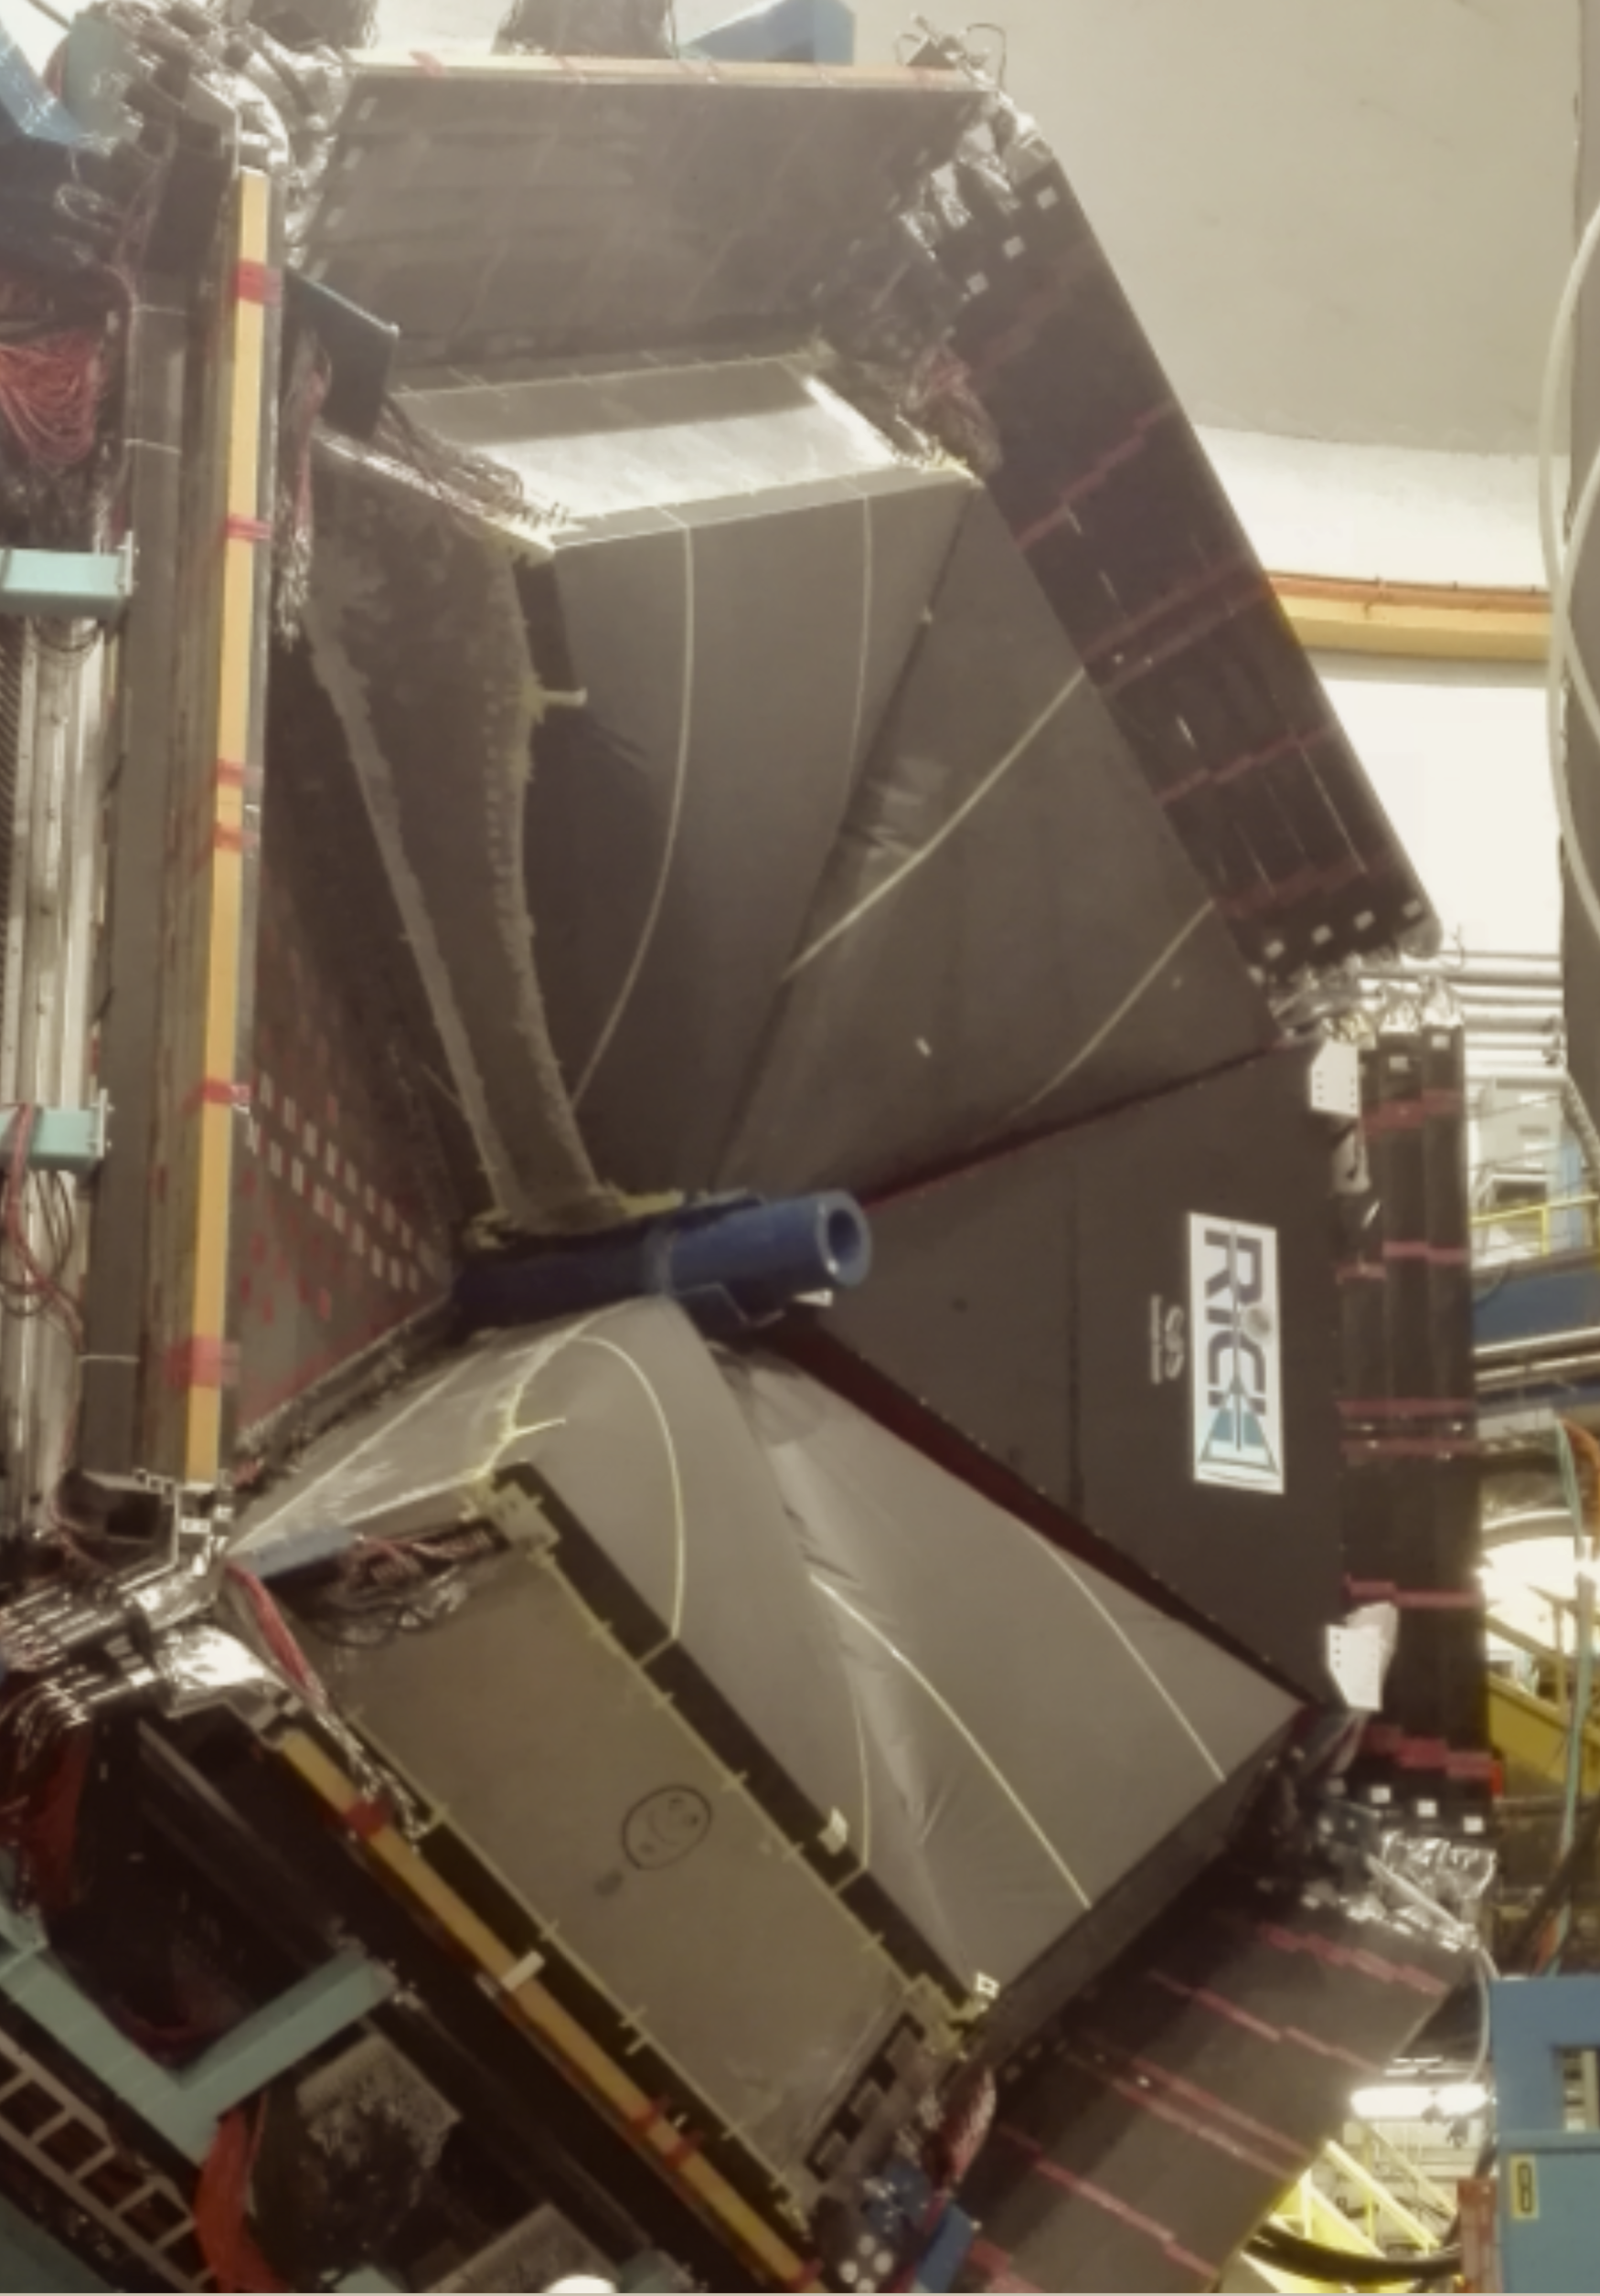
\includegraphics[width=1.0\columnwidth,keepaspectratio]{img/ltccInstalled.png}
    \caption{The LTCC sectors installed after refurbishment on the CLAS12 Forward Carriage. The RICH detector
    is installed in the sector~4 position and the sector~1 position awaits the installation of a second RICH detector.}
    \label{fig:ltccInstalled}
\end{figure}

\section{Acknowledgments}

We thank the Detector Support Group at Jefferson Lab for the work on the cone refurbishment, reflectivity tests,
PMT divider modifications and installation, and for designing the gas control system and associated software. We
thank Temple University for the p-terphenyl deposition. We thank Vladimir Popov for the implementation of the
divider base modification. We thank Youri Sharabian and Steve Christo for their consultations and contributions.
We thank the technical team of Hall~B for their work and dedication on all aspect of the project. Finally, we thank
all the Hall~B staff for their unyielding support. This work was supported in part by
DOE Contract DE-AC05-84ER40150.

\section{References}

%%\bibliography{bibfile}
%%\bibliographystyle{elsarticle-num}


\begin{thebibliography}{99}

\bibitem{daq-ref}
S.~Boyarinov {\it et al.}, {\it ``The CLAS12 Data Acquisition System''}, see this issue.

%@article{ssp-ref,
%	title = "{The SSP Board}",
%	author = "Benjamin Raydo, 14 January 2014",
%	url = "https://coda.jlab.org/drupal/system/files/pdfs/HardwareManual/SSP/SSP_Module_HallD_v1.2.pdf"
%}

%@article{vtp-ref,
%	title = "{The VTP Board}",
%	author = "Benjamin Raydo, September 2016",
%	url = "fhttps://coda.jlab.org/drupal/system/files/pdfs/HardwareManual/VTP/VTP-HallB-Manual.pdf"
%}

\bibitem{overview-ref}
V.D.~Burkert {\it et al.}, {\it ``The CLAS12 Spectrometer at Jefferson Laboratory''}, see this issue.

\bibitem{clas-nim}
B.A.~Mecking {\it et al.}, Nucl. Inst. and Meth. {\bf A503}, 513 (2003).

\bibitem{cnd-ref}
J. Bettane {\it et al.}, {\it ``The CLAS12 Central Neutron Detector''}, see this issue.

\bibitem{ftof-ref}
D.S. Carman {\it et al.}, {\it ``The Forward Time-of-Flight System for CLAS12''}, see this issue.

\bibitem{ctof-ref}
D.S. Carman {\it et al.}, {\it ``The Central Time-of-Flight System for CLAS12''}, see this issue.

\bibitem{htcc-ref}
Y. Sharabian {\it et al.}, {\it ``The CLAS12 High Threshold Cherenkov Counter''}, see this issue.

\bibitem{ec-ref}
G. Asryan {\it et al.}, {\it ``The CLAS12 Forward Electromagnetic Calorimeter''}, see this issue.

\bibitem{dc-ref}
M. Mestayer {\it et al.}, {\it ``The CLAS12 Drift Chamber System''}, see this issue.

\bibitem{gemc-ref}
M. Ungaro {\it et al.}, {\it ``The CLAS12 Geant4 Simulation''}, see this issue.

\bibitem{offline-ref}
V. Ziegler {\it et al.}, {\it ``The CLAS12 Event Reconstruction'}, see this issue.

\bibitem{ft-ref}
NNN {\it et al.}, {\it ``The CLAS12 Forward Tagger System''}, see this issue.

\bibitem{hls-ref}
HLS {\it et al.}, {\it ``VIVAO High Level Synthesis''}, yyy.

\end{thebibliography}


\end{document}








